\documentclass[tikz,border=10pt]{standalone}


\begin{document}
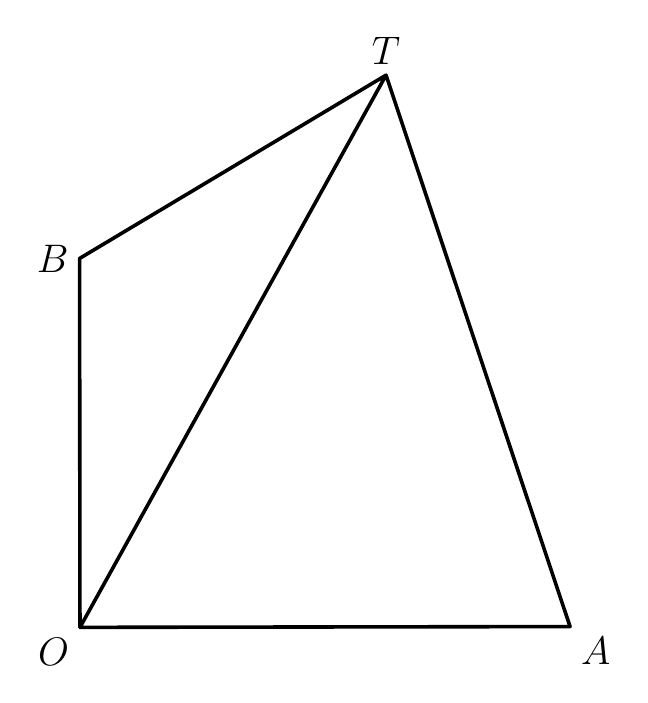
\begin{tikzpicture}[line width=1.3pt, line join=round]
\coordinate (A) at (3.285,-3.497);
\coordinate (B) at (-2.944,1.178);
\coordinate (O) at (-2.939,-3.507);
\coordinate (T) at (0.948,3.506);

  
  \draw (O) -- (A) -- (T) -- (B) -- (O) -- (T);

  
  \node[above, font=\fontsize{14}{16.8}\selectfont] at (T) {$T$};
  \node[left, font=\fontsize{14}{16.8}\selectfont] at (B) {$B$};
  \node[below left, font=\fontsize{14}{16.8}\selectfont] at (O) {$O$};
  \node[below right, font=\fontsize{14}{16.8}\selectfont] at (A) {$A$};
\end{tikzpicture}
\end{document}